\documentclass[12pt,journal]{IEEEtran}
\usepackage{color}
\ifCLASSINFOpdf
  \usepackage[pdftex]{graphicx}
  % declare the path(s) where your graphic files are
  % \graphicspath{{../pdf/}{../jpeg/}}
  % and their extensions so you won't have to specify these with
  % every instance of \includegraphics
  % \DeclareGraphicsExtensions{.pdf,.jpeg,.png}
\else
  % or other class option (dvipsone, dvipdf, if not using dvips). graphicx
  % will default to the driver specified in the system graphics.cfg if no
  % driver is specified.
  % \usepackage[dvips]{graphicx}
  % declare the path(s) where your graphic files are
  % \graphicspath{{../eps/}}
  % and their extensions so you won't have to specify these with
  % every instance of \includegraphics
  % \DeclareGraphicsExtensions{.eps}
\fi
\usepackage{pgfplots}
\usepackage{cite}
\usepackage{subcaption}
\usepackage[boxed]{algorithm2e}

\begin{document}

\newcommand{\todo}[1]{{\color{red} #1}}

\title{Implementation of a Spam Filter}
\author{Michael Aquilina, Student no.: 1329899, Account: ma13673 \\
    Uwe Korn, Student no.: 1348203, Account: uk13734}
\maketitle
\IEEEpeerreviewmaketitle

\section{Introduction}
\todo{Write me!}

\todo{Crossvalidation: 10fold, Confusion matrix is sum over all folds}

\todo{Which quality measure did we choose?}



\section{Naive Bayes}
A Naive Bayes implementation was developed as Part 1 of our report and will be used as our classifier throughout the report.
We shall be using the Bag of Words model to extract features from the emails which treats each independent word in the document corpus as an individual feature.
Our specific implementation of Naive Bayes makes use of a multinomial distribution in its underlying model which takes the frequency of each word as its distribution rather than the binary value of simple existence.
It is important to note that the in general, Naive Bayes models make the assumption that words are independently drawn from each other and does not model any dependencies between them.

The probabilities generated during training and classification are always stored as log-likelihoods to minimize numerical errors.
Due to the low number of numerical errors, the Naive Bayes implementation was able to cope with a large number of 143820 dimensions (i.e. number of different words in the input data) as its initial feature set.

To obtain an initial baseline performance, we ran the Naive Bayes classifier on the training set using 10-fold cross validation.
This resulted in an accuracy of 0.944 and a standard deviation across all folds of 0.024 for the Naive Bayes classifier without using the underlying class distribution as a-priori probabilities.
With the usage of the underlying distribution, we get a classification accuracy of 0.9472 and a standard deviation of 0.032.

Although the class distribution (81\% Ham, 19\% Spam) is very different to a uniform distribution, the resulting classification score is not significantly different.
\todo{clarify this section}With each instantiation taking 16 minutes to train and classify, the runtime does not make a difference either as the feature size stayed the same.
\todo{As using maximum-a-posteriori is the most common used Naive Bayes approach, we are going to use it in the following as our baseline which we will optimise using various preprocessing techniques.}



\section{Preprocessing}
The bag of words model used by our classifiers is a good way to represent the data found in the given training documents. However this feature representation is prone to very high dimensions if not handled well due to the large number of possible combinations in words. 

According to a recent survey performed by Google and Harvard, there are approximately 1,022,000 different words in the English language \cite{google2010words}. While we do not expect to find all possible words in the document corpus, a large number of them will be found along with their derivations in the form of spelling mistakes and grammatical variations (e.g.{\it they're} and {\it theyre}). Other non-English words such as html code, URLs and nonsensical data such as GPG keys will also be found within the documents.

Most of these words will provide no benefit to the classifier and in most cases will even harm the classifier's performance. It is therefore of utmost importance that noise in the text is filtered out and the number of word combinations is reduced to the most representative, yet minimal subset of the available words. The following steps are taken to do this:
\begin{itemize}
	\item Smart Email Parsing
	\item Simple Text Processing Techniques
	\item Domain Extraction
	\item Stemming
	\item Feature Selection based on Document Frequency
\end{itemize}

Each of these steps contribute towards achieving a higher accuracy and performance in the classifier and will be described in detail in the sections below.

\subsection{Email Parsing}
As a first preprocessing step, we modify the parsing of the email structure.
The provided emails sometimes contain metadata which is very redundant w.r.t. to the number of contained words, e.g. all will have a "From" line but also if an email has metadata is independent from its class label, i.e. the classifier should not that all mails that have metadata are spam.
Furthermore mails do not always consist of just text but also have attachments or their textual content is supplied as plain text or beautified with HTML markup.

In a first step, we strip the metadata from the email so that only give the content of the mail to the classifier.
This reduces the size of data passed on to the classifier as most terms in the metadata are either common among all emails, e.g. the names of the header lines (``From'', ``Content-Type'', \dots), or are unique to the mail like the date of sending or the message-id.
From the metadata we extract some basic information like the encoding or if it is a multi-part email for further processing.

If the mail is split in multiple parts, we want to extract only the parts which contain text as we cannot infer information of the \emph{base64} representation of images or other binary attachments.
These binary attachments would only add a large number of words of a length of 76 characters \cite{rfc2045} to the index which are very uncommon in other mails as images are compressed data with a high entropy.
Another problem that is solved by adding handling multiple is the recursive parsing of attached emails that have textual content and may have multiple parts again inside so that we are now stripping down the inner mails to their actual content too.

Furthermore not all text is encoded in the same encoding as the email itself, e.g. the main text could be encoded as Base64 which would not reveal the actual words when just splitting the mail into words by separating at each space.
Another typical encoding is quoted-printable which only transforms non-ASCII characters into another format but leaves all ASCII characters intact.
Handling these encoding turns meaningless, long character sequences into words that are present in other mails.

As a final parsing step in the email handling we are stripping all HTML from the mails to remove all HTML tags from our word index.
This markup is not displayed to the user and does not carry any content that will be some sort of advertising.

Although email parsing did not make a significant impact on the quality score of the classifier, it reduced its dimensionality from 143820 down to 94903.
With this lower dimensionality the runtime decreases too from 16 minutes to ten.
In conclusion email parsing stripped a lot of irrelevant or redundant dependencies from the input data set without the cost of quality loss.

\subsection{Simple Text Processing Techniques}

A number of simple processing techniques are used to conflate incoming strings that represent the word together. Although the email parser is built in such a way as to strip out html content where possible, a number of artefacts could still linger in the data which could cause noise and incorrectly distinguish variations of the same word. Because it is not the parsers job to perform this form of filtering, a separate step is taken to perform simple text processing tasks before passing them on the later pre-processing stages.

All incoming words that are composed purely of symbols (i.e. no numbers or letters) are simply discarded as they are most commonly noise in the data that does not represent anything in the corpus. Without this step, the number of features used by the classifier would grow substantially as a large number of "rubbish" symbols are included as part of the feature set. Additionally, all remaining words will have ally symbols stripped, this prevents variations in words like {\it they're} and {\it theyre} from being treated as different features.

As a second step, all valid incoming words are simply reduced to lower-case format. The same word in different cases should not be distinguished from one another during classification so it is important that e.g. {\it Bristol} is considered the same as {\it bristol}.

Finally, variations in number representations (e.g. 4,000 and 4000) are detected using regular expressions and conflated to a single representative feature "9999". We do this because allowing all possible number combinations each a unique feature will increase the dimensionality substantially and rarely contribute to classification performance - it can most often be considered noise. Doing this also provides some assurance that we do not overfit our classifier to the training set with specific numeric combinations.

Using the techniques described above we were able to reduce the number of  combinations from 94,903 words to just 56149. This is a substantial decrease in dimensions and provides a very notable improvement to memory usage, training speed and classification speed. 

\todo{note that accuracy increases to 97.4 from 95.1?}

\subsection{Domain Extraction}

Due to the fact that Emails are a product of the web, it is very common to find items representing Uniform Resource Locaters (URLs) and email addresses within the their text. When left unprocessed, it is hard to group these items into corresponding features due to additional data included within them.

What we really care about is the domain each URL and email address contains. If we find two URLs which point to the same domain such as {\it www.cs.bris.ac.uk/maths} and {\it www.cs.bris.ac.uk/eng}, the it would make sense to group these two items together as one feature - i.e. coming from the domain {\it cs.bris.ac.uk}. This will prove useful in being able to identify URLs which point to malicious or spam websites and those which are well known and credible domains.

To do this, we use a regular expression parser to detect items that are URLs and email addresses. Detected items are put through a {\it Domain Extraction} function which is able to strip out the username and '@' symbol in the case of emails (e.g. {\it johndoe@example.com} would become {\it example.com}) and remove paths and protocol declerations in the case of URLs (e.g. {\it https://www.example.com/myimage.jpg} would become {\it example.com} once again). Conflating both email address domains and web URL domains makes sense because they represent the same source of information.


\subsection{Stemming}
Most words in the English language are derived from a {\it morphological root} word that contains no prefixes or suffixes and conveys a very similar meaning to its derivation. A simple example of this is {\it subscriber} and {\it subscription} with their morphological root {\it subscribe}. 

If we can reduce all incoming words into their root form, we would be able to substantially reduce the number of dimensions for our model while also ensuring that words representing the same underlying feature are stored under the same value.

Unfortunately, such a task is quite hard and would probably require the creation of a very large lookup table for each word in the English language along with its root. This is due to the fact that the English language is not a formal language and hence does not follow a strict set of rules. 

We could however, take an approximation of the described process and instead derive the {\it stem} of each word. Like the morphological root, the stem is a representation of a words underlying meaning. However the stem does not guarantee to be a correct English word or generate the right root as its aim is simply to map variations of the same word to the same to item. 

For our Spam Filter implementation, we made use of the Porter Stemmer algorithm \cite{porter1980}, which in the authors words is ``a process for removing the commoner morphological and inflexional endings from words in English''. In simpler terms, it is capable of removing known suffixes from words passed to it. The Porter Stemmer algorithm is available as open source code under the BSD License and is available in multiple languages, including Java which is made use of in our implementation.

Using the same examples shown before, passing {\it subscriber} and {\it subscribe} to the Porter Stemmer would reduce the words {\it subscribe} and {\it subscriber} to the stem {\it subscrib}. On the other hand, the word {\it subscription} will be wrongly mapped to a different stem - {\it subscript}. The latter is an example of where the approximation fails to produce the correct result, however in general most words passed to the algorithm have shown to produce favourable results.

In terms of the Spam Filter implementation, using Porter Stemming on the given set of training emails reduced the number of words from 24813 words to 18932 stems (both after text pre-processing). This is a substantial reduction in the number of dimensions and plays a crucial role in ensuring that the classifier is able to train with the given documents in a short amount of time and without requiring large amounts of memory. Apart from improving speed and reducing memory, it has also proved to improve classification performance. \todo{include some results - simple example I have is 0.973 with and 0.97 without}.

\todo{Improvement?}

\subsection{Feature selection}
\todo{Is this really preprocessing?}

As the number of features generated by the input data is even very high after the previous preprocessing steps, we are going to minimise its number by trimming features which are (significantly) relevant for the classification quality.

\todo{\dots}

\begin{figure}[h!]
    \centering
    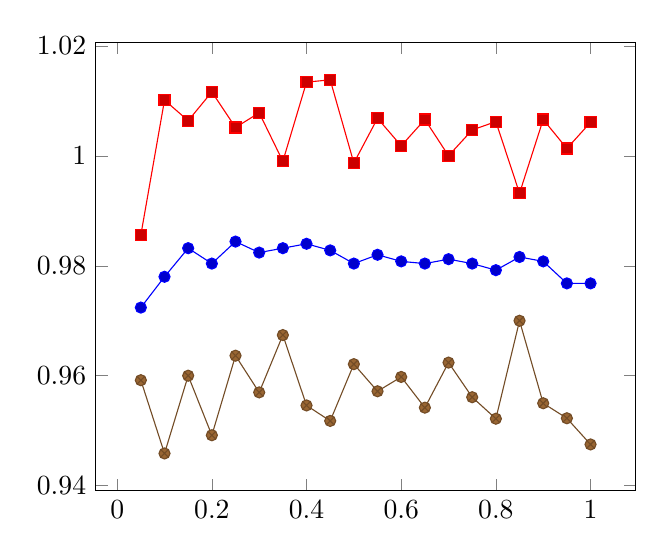
\begin{tikzpicture}
        \begin{axis}
             \addplot+[sharp plot] coordinates {
                (0.05, 0.972400)
                (0.10, 0.978000)
                (0.15, 0.983200)
                (0.20, 0.980400)
                (0.25, 0.984400)
                (0.30, 0.982400)
                (0.35, 0.983200)
                (0.40, 0.984000)
                (0.45, 0.982800)
                (0.50, 0.980400)
                (0.55, 0.982000)
                (0.60, 0.980800)
                (0.65, 0.980400)
                (0.70, 0.981200)
                (0.75, 0.980400)
                (0.80, 0.979200)
                (0.85, 0.981600)
                (0.90, 0.980800)
                (0.95, 0.976800)
                (1.00, 0.976800)
                };
             \addplot+[sharp plot] coordinates {
                (0.05, 0.972400+0.013206)
                (0.10, 0.978000+0.032125)
                (0.15, 0.983200+0.023186)
                (0.20, 0.980400+0.031215)
                (0.25, 0.984400+0.020746)
                (0.30, 0.982400+0.025424)
                (0.35, 0.983200+0.015799)
                (0.40, 0.984000+0.029394)
                (0.45, 0.982800+0.031010)
                (0.50, 0.980400+0.018287)
                (0.55, 0.982000+0.024819)
                (0.60, 0.980800+0.021014)
                (0.65, 0.980400+0.026199)
                (0.70, 0.981200+0.018804)
                (0.75, 0.980400+0.024298)
                (0.80, 0.979200+0.027011)
                (0.85, 0.981600+0.011593)
                (0.90, 0.980800+0.025799)
                (0.95, 0.976800+0.024528)
                (1.00, 0.976800+0.029285)
                };
             \addplot+[sharp plot] coordinates {
                (0.05, 0.972400-0.013206)
                (0.10, 0.978000-0.032125)
                (0.15, 0.983200-0.023186)
                (0.20, 0.980400-0.031215)
                (0.25, 0.984400-0.020746)
                (0.30, 0.982400-0.025424)
                (0.35, 0.983200-0.015799)
                (0.40, 0.984000-0.029394)
                (0.45, 0.982800-0.031010)
                (0.50, 0.980400-0.018287)
                (0.55, 0.982000-0.024819)
                (0.60, 0.980800-0.021014)
                (0.65, 0.980400-0.026199)
                (0.70, 0.981200-0.018804)
                (0.75, 0.980400-0.024298)
                (0.80, 0.979200-0.027011)
                (0.85, 0.981600-0.011593)
                (0.90, 0.980800-0.025799)
                (0.95, 0.976800-0.024528)
                (1.00, 0.976800-0.029285)
                };
    \end{axis}
    \end{tikzpicture}
    \caption{Accuracy w.r.t. upper threshold (lower threshold = 0)}
    \label{p:upperbound}
\end{figure}



\begin{figure}[h!]
    \centering
    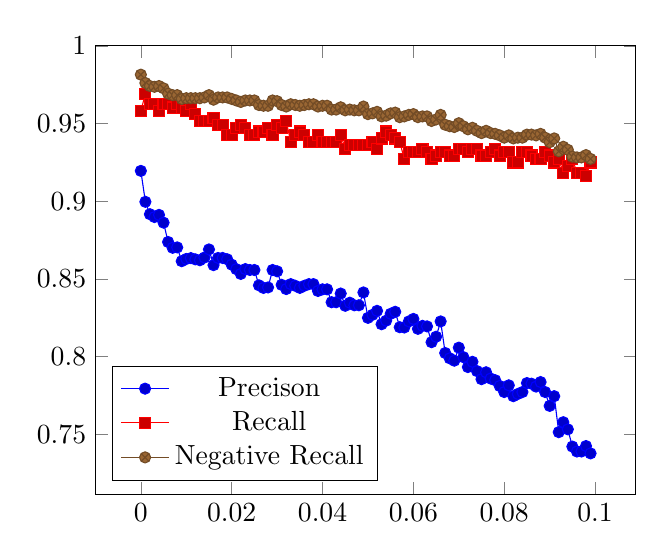
\begin{tikzpicture}
        \begin{axis}[
                legend pos=south west,
                ymax=1,
                xtick={0, 0.02, 0.04, 0.06, 0.08, 0.1},
                xticklabels={0, 0.02, 0.04, 0.06, 0.08, 0.1}
                ]
                \addplot+[sharp plot] coordinates {
                    (0.0, 0.919492)
                    (0.001, 0.899590)
                    (0.002, 0.891616)
                    (0.003, 0.889796)
                    (0.004, 0.891170)
                    (0.005, 0.886179)
                    (0.006, 0.873747)
                    (0.007, 0.870000)
                    (0.008, 0.870259)
                    (0.009, 0.861386)
                    (0.010, 0.862823)
                    (0.011, 0.863366)
                    (0.012, 0.862550)
                    (0.013, 0.862000)
                    (0.014, 0.863727)
                    (0.015, 0.868952)
                    (0.016, 0.858847)
                    (0.017, 0.863454)
                    (0.018, 0.863454)
                    (0.019, 0.862626)
                    (0.020, 0.859155)
                    (0.021, 0.856287)
                    (0.022, 0.853175)
                    (0.023, 0.856287)
                    (0.024, 0.855711)
                    (0.025, 0.855711)
                    (0.026, 0.845850)
                    (0.027, 0.844181)
                    (0.028, 0.844488)
                    (0.029, 0.855711)
                    (0.030, 0.854871)
                    (0.031, 0.846154)
                    (0.032, 0.843444)
                    (0.033, 0.846614)
                    (0.034, 0.845545)
                    (0.035, 0.844181)
                    (0.036, 0.845545)
                    (0.037, 0.846614)
                    (0.038, 0.846614)
                    (0.039, 0.842209)
                    (0.040, 0.843254)
                    (0.041, 0.843254)
                    (0.042, 0.834971)
                    (0.043, 0.834971)
                    (0.044, 0.840551)
                    (0.045, 0.832677)
                    (0.046, 0.834646)
                    (0.047, 0.833006)
                    (0.048, 0.833006)
                    (0.049, 0.841270)
                    (0.050, 0.824903)
                    (0.051, 0.826848)
                    (0.052, 0.829412)
                    (0.053, 0.820809)
                    (0.054, 0.823077)
                    (0.055, 0.827519)
                    (0.056, 0.828794)
                    (0.057, 0.818882)
                    (0.058, 0.818713)
                    (0.059, 0.822612)
                    (0.060, 0.824219)
                    (0.061, 0.817829)
                    (0.062, 0.819767)
                    (0.063, 0.819417)
                    (0.064, 0.809249)
                    (0.065, 0.812741)
                    (0.066, 0.822612)
                    (0.067, 0.802281)
                    (0.068, 0.798861)
                    (0.069, 0.797348)
                    (0.070, 0.805714)
                    (0.071, 0.799622)
                    (0.072, 0.793233)
                    (0.073, 0.796610)
                    (0.074, 0.790654)
                    (0.075, 0.785448)
                    (0.076, 0.789869)
                    (0.077, 0.785847)
                    (0.078, 0.784787)
                    (0.079, 0.781076)
                    (0.080, 0.777164)
                    (0.081, 0.781481)
                    (0.082, 0.774492)
                    (0.083, 0.775926)
                    (0.084, 0.777164)
                    (0.085, 0.782931)
                    (0.086, 0.782528)
                    (0.087, 0.780669)
                    (0.088, 0.783582)
                    (0.089, 0.777164)
                    (0.090, 0.768248)
                    (0.091, 0.774492)
                    (0.092, 0.751342)
                    (0.093, 0.757741)
                    (0.094, 0.753153)
                    (0.095, 0.742049)
                    (0.096, 0.738899)
                    (0.097, 0.738899)
                    (0.098, 0.742397)
                    (0.099, 0.737676)
            };
        \addlegendentry{Precison}
        \addplot+[sharp plot] coordinates {
            (0.0, 0.958057)
                (0.001, 0.969095)
                (0.002, 0.962472)
                (0.003, 0.962472)
                (0.004, 0.958057)
                (0.005, 0.962472)
                (0.006, 0.962472)
                (0.007, 0.960265)
                (0.008, 0.962472)
                (0.009, 0.960265)
                (0.010, 0.958057)
                (0.011, 0.962472)
                (0.012, 0.955850)
                (0.013, 0.951435)
                (0.014, 0.951435)
                (0.015, 0.951435)
                (0.016, 0.953642)
                (0.017, 0.949227)
                (0.018, 0.949227)
                (0.019, 0.942605)
                (0.020, 0.942605)
                (0.021, 0.947020)
                (0.022, 0.949227)
                (0.023, 0.947020)
                (0.024, 0.942605)
                (0.025, 0.942605)
                (0.026, 0.944812)
                (0.027, 0.944812)
                (0.028, 0.947020)
                (0.029, 0.942605)
                (0.030, 0.949227)
                (0.031, 0.947020)
                (0.032, 0.951435)
                (0.033, 0.938190)
                (0.034, 0.942605)
                (0.035, 0.944812)
                (0.036, 0.942605)
                (0.037, 0.938190)
                (0.038, 0.938190)
                (0.039, 0.942605)
                (0.040, 0.938190)
                (0.041, 0.938190)
                (0.042, 0.938190)
                (0.043, 0.938190)
                (0.044, 0.942605)
                (0.045, 0.933775)
                (0.046, 0.935982)
                (0.047, 0.935982)
                (0.048, 0.935982)
                (0.049, 0.935982)
                (0.050, 0.935982)
                (0.051, 0.938190)
                (0.052, 0.933775)
                (0.053, 0.940397)
                (0.054, 0.944812)
                (0.055, 0.942605)
                (0.056, 0.940397)
                (0.057, 0.938190)
                (0.058, 0.927152)
                (0.059, 0.931567)
                (0.060, 0.931567)
                (0.061, 0.931567)
                (0.062, 0.933775)
                (0.063, 0.931567)
                (0.064, 0.927152)
                (0.065, 0.929360)
                (0.066, 0.931567)
                (0.067, 0.931567)
                (0.068, 0.929360)
                (0.069, 0.929360)
                (0.070, 0.933775)
                (0.071, 0.933775)
                (0.072, 0.931567)
                (0.073, 0.933775)
                (0.074, 0.933775)
                (0.075, 0.929360)
                (0.076, 0.929360)
                (0.077, 0.931567)
                (0.078, 0.933775)
                (0.079, 0.929360)
                (0.080, 0.931567)
                (0.081, 0.931567)
                (0.082, 0.924945)
                (0.083, 0.924945)
                (0.084, 0.931567)
                (0.085, 0.931567)
                (0.086, 0.929360)
                (0.087, 0.927152)
                (0.088, 0.927152)
                (0.089, 0.931567)
                (0.090, 0.929360)
                (0.091, 0.924945)
                (0.092, 0.927152)
                (0.093, 0.918322)
                (0.094, 0.922737)
                (0.095, 0.927152)
                (0.096, 0.918322)
                (0.097, 0.918322)
                (0.098, 0.916115)
                (0.099, 0.924945)
        };
        \addlegendentry{Recall}
        \addplot+[sharp plot] coordinates {
            (0.0, 0.981436)
            (0.001, 0.976063)
            (0.002, 0.974108)
            (0.003, 0.973620)
            (0.004, 0.974108)
            (0.005, 0.972643)
            (0.006, 0.969223)
            (0.007, 0.968246)
            (0.008, 0.968246)
            (0.009, 0.965804)
            (0.010, 0.966292)
            (0.011, 0.966292)
            (0.012, 0.966292)
            (0.013, 0.966292)
            (0.014, 0.966781)
            (0.015, 0.968246)
            (0.016, 0.965315)
            (0.017, 0.966781)
            (0.018, 0.966781)
            (0.019, 0.966781)
            (0.020, 0.965804)
            (0.021, 0.964827)
            (0.022, 0.963850)
            (0.023, 0.964827)
            (0.024, 0.964827)
            (0.025, 0.964827)
            (0.026, 0.961895)
            (0.027, 0.961407)
            (0.028, 0.961407)
            (0.029, 0.964827)
            (0.030, 0.964338)
            (0.031, 0.961895)
            (0.032, 0.960918)
            (0.033, 0.962384)
            (0.034, 0.961895)
            (0.035, 0.961407)
            (0.036, 0.961895)
            (0.037, 0.962384)
            (0.038, 0.962384)
            (0.039, 0.960918)
            (0.040, 0.961407)
            (0.041, 0.961407)
            (0.042, 0.958964)
            (0.043, 0.958964)
            (0.044, 0.960430)
            (0.045, 0.958476)
            (0.046, 0.958964)
            (0.047, 0.958476)
            (0.048, 0.958476)
            (0.049, 0.960918)
            (0.050, 0.956033)
            (0.051, 0.956522)
            (0.052, 0.957499)
            (0.053, 0.954568)
            (0.054, 0.955056)
            (0.055, 0.956522)
            (0.056, 0.957010)
            (0.057, 0.954079)
            (0.058, 0.954568)
            (0.059, 0.955545)
            (0.060, 0.956033)
            (0.061, 0.954079)
            (0.062, 0.954568)
            (0.063, 0.954568)
            (0.064, 0.951637)
            (0.065, 0.952614)
            (0.066, 0.955545)
            (0.067, 0.949194)
            (0.068, 0.948217)
            (0.069, 0.947728)
            (0.070, 0.950171)
            (0.071, 0.948217)
            (0.072, 0.946263)
            (0.073, 0.947240)
            (0.074, 0.945286)
            (0.075, 0.943820)
            (0.076, 0.945286)
            (0.077, 0.943820)
            (0.078, 0.943332)
            (0.079, 0.942355)
            (0.080, 0.940889)
            (0.081, 0.942355)
            (0.082, 0.940401)
            (0.083, 0.940889)
            (0.084, 0.940889)
            (0.085, 0.942843)
            (0.086, 0.942843)
            (0.087, 0.942355)
            (0.088, 0.943332)
            (0.089, 0.940889)
            (0.090, 0.937958)
            (0.091, 0.940401)
            (0.092, 0.932096)
            (0.093, 0.935027)
            (0.094, 0.933073)
            (0.095, 0.928676)
            (0.096, 0.928188)
            (0.097, 0.928188)
            (0.098, 0.929653)
            (0.099, 0.927211)
        };
        \addlegendentry{Negative Recall}
        \end{axis}
    \end{tikzpicture}
    \caption{Precision and recall w.r.t. lower threshold (no cap on the upper bound)}
    \label{p:lowerbound}
\end{figure}



\todo{explain what each line in the figure represents and make sure standard deviation is calculated correctly (it should not go above 1.0)..}


\section{Alternatives to Naive Bayes}
As a classifier is modeld after some given assumptions and with specific architechtural properities, e.g. all attributes are equally important, it is important to check if the used classifier is the right model for the examined problem.
A very good feature of the Naive Bayes classifier is its ability to train on a dataset with a very high dimensionality in decent time.
Because this property is not shared among all other classifier and some even severely suffer from high dimensionality (the so called Curse of Dimensionality \cite{bellman1957dynamic}), we are using the reduced set of features we estimated in the feature selection process without further research on the impact of other thresholds on feature trimming w.r.t. to non-bayesian classifiers.

\subsection{Decision Trees}

We are going to use Weka's \cite{hall2009weka} implementation of the C4.5 decision tree \cite{Quinlan1993} (known in Weka as J48) as the first alternative to Naive Bayes classification.
C4.5 builts a tree based on the features using information entropy.
The dimension with the highest information gain will be used at each node new to generate a new split.
After the creation of the tree, C4.5 tries to prune all unnecessary branches with leafs to keep the total number of nodes to a minimum.
Altough this feature could be disabled, we are using it to avoid overfitting.

As the runtime of C4.5 increases in a higher level with the number of dimensions than the Naive Bayes Classifier, we are going to use it with the threshold $\alpha=0.017$ and $\beta=0.19$.
This reduced data set of only 1568 dimensions can be used to train a C4.5 tree in a feasible amount of timeThis reduced data set of only 1568 dimensions can be used to train a C4.5 tree in a feasible amount of time.

\begin{figure}[h!]
    \centering
    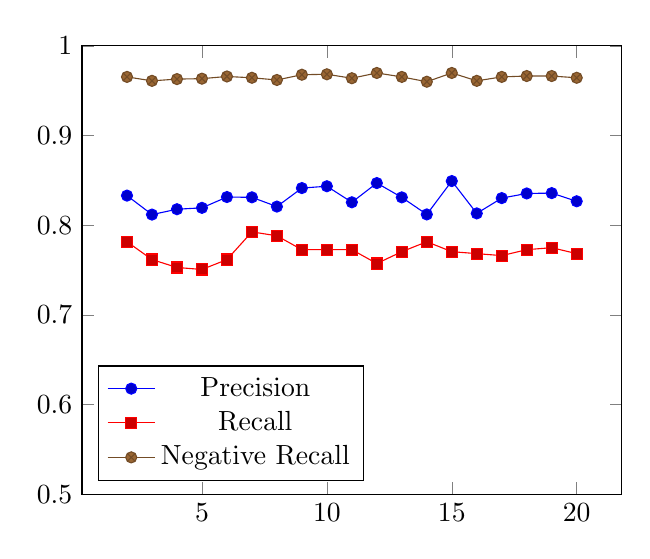
\begin{tikzpicture}
        \begin{axis}[
            legend pos=south west,
            ymax=1,
            ymin=0.5
            ]
            \addplot+[sharp plot] coordinates {
            (2, 0.832941)
            (3, 0.811765)
            (4, 0.817746)
            (5, 0.819277)
            (6, 0.831325)
            (7, 0.831019)
            (8, 0.820690)
            (9, 0.841346)
            (10, 0.843373)
            (11, 0.825472)
            (12, 0.846914)
            (13, 0.830952)
            (14, 0.811927)
            (15, 0.849148)
            (16, 0.813084)
            (17, 0.830144)
            (18, 0.835322)
            (19, 0.835714)
            (20, 0.826603)
            };
            \addlegendentry{Precision}
            \addplot+[sharp plot] coordinates {
            (2, 0.781457)
            (3, 0.761589)
            (4, 0.752759)
            (5, 0.750552)
            (6, 0.761589)
            (7, 0.792494)
            (8, 0.788079)
            (9, 0.772627)
            (10, 0.772627)
            (11, 0.772627)
            (12, 0.757174)
            (13, 0.770419)
            (14, 0.781457)
            (15, 0.770419)
            (16, 0.768212)
            (17, 0.766004)
            (18, 0.772627)
            (19, 0.774834)
            (20, 0.768212)
            };
            \addlegendentry{Recall}
            \addplot+[sharp plot] coordinates {
            (2, 0.965315)
            (3, 0.960918)
            (4, 0.962872)
            (5, 0.963361)
            (6, 0.965804)
            (7, 0.964338)
            (8, 0.961895)
            (9, 0.967758)
            (10, 0.968246)
            (11, 0.963850)
            (12, 0.969712)
            (13, 0.965315)
            (14, 0.959941)
            (15, 0.969712)
            (16, 0.960918)
            (17, 0.965315)
            (18, 0.966292)
            (19, 0.966292)
            (20, 0.964338)
            };
            \addlegendentry{Negative Recall}
        \end{axis}
    \end{tikzpicture}
    \caption{Performance of J48 w.r.t. the number of minimum instances per leaf}
    \label{fig:j48}
\end{figure}



One of the parameters that can be adjusted is the number of instances each leaf of the tree needs to represent at least during the training phase.
The default setting of WEKA requires at minimum two instances at each leaf, in Figure \ref{fig:j48} we outline the scores with varying number of minimum instances.
From the results we can see that chaging the minimum number of instances has not a large impact on the score of the classifier.
Because of this we are going to use WEKA's default setting of a minimum of two instances per leaf for comparing the performance of J48 to our best Naive Bayes instantiation.

To compare the performance of both classifiers, we are testing the null hypothesis that they generate equal good results.
The testing will be done using 10-fold crossvalidation on the same training set and the statistical significance of the results will be examined using Wilcoxon's signed-rank-test.
As we already have used different measures throughout the whole document, we will be testing the performance of both classifiers using \emph{Accuracy}, \emph{Precision} and \emph{Recall}.
For the statistical test, we are using 5\% as our confidence level, i.e. to successfully reject the null hypothesis that both classifiers produce similar results, the minimum sum of positive or negative ranks must be eight or less.

\begin{table}[h!]
    \centering
    \begin{tabular}{ | l | r | r | }
        \hline
        \textbf{Measure} & \textbf{Difference} & $\min(\sum +ranks, \sum -ranks)$ \\
        \hline
        \emph{Accuracy} & 0.048 & 0 \\
        \hline
        \emph{Precision} & 0.111 & 1 \\
        \hline
        \emph{Recall} & 0.167 & 0 \\
        \hline
    \end{tabular}
    \caption{Average differences in the quality scores and minimum sum of either positive or negative ranks of Naive Bayes and J48 based on 10-fold cross validation}
    \label{table:difference}
\end{table}

Table \ref{table:difference} shows the average differences between both classifiers and shows clearly that that on average Naive Bayes performs better.
With all ranks below $8$, we can reject the null hypothesis for all measures that the classifiers produce similar results.
As the scores of Naive Bayes were always better, we can conclude that Naive Bayes outperforms C4.5/J48 for our dataset of Spam data for the given feature vectors.
Remarkably J48 could only outperform Naive Bayes in one fold and in this fold it was only better in \emph{Precision} where Naive Bayes still lead to better scores in \emph{Accuracy} and \emph{Recall}.



\section{Conclusion}

The Naive Bayes classifier proved to be a surprisingly efficient machine learning technique despite its aptly given name (It is sometimes even lovingly referred to as Idiots Bayes due to its simplicity \cite{idiotsbayes2001}).
It has proven to output results with high accuracy, precision and recall - even outperforming more advanced machine learning techniques such as Decision Trees.
With a final accuracy of 0.984 and precision of 96.8 calculated through cross validation, our email classifier should correctly distinguish between ham and spam emails on a number of different test sets.

Future work can be done to both improve pre-processing techniques by further analysing meta-data within the headers and including additional text processing techniques such as spell correction to conflate words further into their respective features. Further natural language processing techniques can also be attempted on the text and a comparison in performance to the Bernoulli model for Naive Bayes can also be attempted in future work.



\bibliography{report}
\bibliographystyle{plain}


\end{document}


